\documentclass[11pt]{article}
\usepackage[utf8]{inputenc}
\usepackage[T1]{fontenc}
\usepackage{amsmath}
\usepackage{amsfonts}
\usepackage{amssymb}
\usepackage[version=4]{mhchem}
\usepackage{stmaryrd}
\usepackage{graphicx}
\usepackage[export]{adjustbox}
\graphicspath{ {./images/} }

\begin{document}
Details of the Income Approach to Real Estate Valuation

This lesson details the estimation of cash flows and the estimation of the discount rate for the income approach along with a discussion of taxes and financing costs.

\section*{Cash Flows for the Income Approach}
The value of a commercial property depends on the benefits it can offer to its investors. The benefits are the future incomes or, preferably, cash flows that are expected over the life of the property being held as a standing investment. The income approach to real estate valuation consists of forecasting a property's future expected revenues (e.g., rents) and expenses and then discounting the income, which is revenues minus expenses, at an appropriate rate to find an estimate of the property's value. The income approach, which is comprised of the direct capitalization method and the discounted cash flow method (DCF), is used to appraise the market value of an income producing property. Market value is defined as the present value of an expected cash flow stream.

Since most properties are unlimited in longevity, cash flows are often projected to some horizon point in time, at which a liquidation value is forecasted. Alternatively, a property may be valued using a perpetuity formula. For long-term horizons, annual values and annual discounting are common.

The investment value (IM) or intrinsic value of the property is based on the discounted expected cash flows, $E\left[C F_{t}\right]$, for each time period, $t$, as illustrated in Equation 1 :


\begin{align*}
I V & =\frac{E\left[C F_{1}\right]}{(1+r)}+\frac{E\left[C F_{2}\right]}{(1+r)^{2}}+\cdots+\frac{E\left[C F_{T-1}\right]}{(1+r)^{T-1}}+\frac{E\left[C F_{T}\right]}{(1+r)^{T}}+\frac{N S P}{(1+r)^{T}} \\
& =\sum_{t=1}^{T} \frac{E\left[C F_{t}\right]}{(1+r)^{t}}+\frac{N S P}{(1+r)^{T}} \tag{1}
\end{align*}


The final term in the equation is the present value of the net sale proceeds. The net sale proceeds (NSP) is the expected selling price minus any expected selling expenses arising from the sale of the property at time $T$. In the case of real estate, interim or operating cash flows are usually estimated using the concept of net operating income. Net operating income (NOI) is a measure of periodic earnings that is calculated as the property's rental income minus all expenses associated with maintaining and operating the property. Equating the expected cash flow at time $t, E\left[C F_{t}\right]$, with the net operating income, $E\left[\mathrm{NOI}_{t}\right]$, generates the following equation:


\begin{align*}
I V & =\frac{E\left[N O I_{1}\right]}{(1+r)}+\frac{E\left[N O I_{2}\right]}{(1+r)^{2}}+\cdots+\frac{E\left[N O I_{T-1}\right]}{(1+r)^{T-1}}+\frac{E\left[N O I_{T}\right]}{(1+r)^{T}}+\frac{N S P}{(1+r)^{T}} \\
& =\sum_{t=1}^{T} \frac{E\left[N O I_{t}\right]}{(1+r)^{t}}+\frac{N S P}{(1+r)^{T}} \tag{2}
\end{align*}


We illustrate the income approach with the following example. Suppose that an investor is considering the purchase of an office building. The potential gross income is the gross income that could potentially be received if all offices in the building were occupied. For this example, the potential gross income of the first year of operations has been estimated at $\$ 300,000$. However, it is unlikely that the building will be fully occupied all year round. In the case of commercial properties, there typically needs to be some consideration for possible vacancies and therefore the loss of rental income. The vacancy loss rate is the observed or anticipated rate at which potential gross income is reduced for space that is not generating rental income. The effective gross income is the potential gross income reduced for the vacancy loss rate. Assuming a $10 \%$ vacancy loss rate and no other income, the effective gross income from the building in the first year will be $\$ 300,000-(\$ 300,000 \times$ $0.1)=\$ 270,000$.

To be able to estimate the NOI, the operating expenses arising from the property need to be estimated and then subtracted from the gross income. Operating expenses are non-capital outlays that support rental of the property and can be classified as fixed or variable. Fixed expenses, examples of which are property taxes and property insurance, do not change directly with the level of occupancy of the property. Variable expenses, examples of which are maintenance, repairs, utilities, garbage removal, and supplies, change as the level of occupancy of the property varies. This simplified example does not consider depreciation, which is discussed later. Continuing with the example, assume that fixed and variable expenses were estimated at $\$ 42,000$ and $\$ 75,000$, respectively, for a total operating expense of $\$ 117,000$ for the first year, or $43.3 \%$ of the first-year effective gross income. Therefore, the NOI arising from this property in the first year is estimated to be:


\begin{align*}
\text { NOI }= & (\text { Potential Gross Income }- \text { Vacancy Loss })-\text { Fixed Expenses }  \tag{3}\\
& - \text { Variable Expenses }
\end{align*}


or

$$
\begin{aligned}
\text { NOI } & =\text { Effective Gross Income }- \text { Operating Expenses } \\
& =\$ 270,000-\$ 117,000=\$ 153,000
\end{aligned}
$$

Now, assuming that the investor expects to maintain the property for seven years, that rents are estimated to increase by $4 \%$ per year, that the vacancy loss rate will remain constant at $10 \%$, and that annual operating expenses will continue to represent the same fraction of effective gross income (117/270), the projected annual NOI for each year in the seven-year period is as shown in the next exhibit.

Finally, assume that the net sale proceeds in year 7 have been estimated at $\$ 1,840,000$.

Estimates of Annual Net Operating Income

\begin{center}
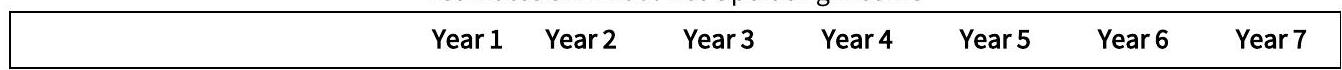
\includegraphics[max width=\textwidth]{2024_04_11_c27706e1a01854b6f538g-2}
\end{center}

\begin{center}
\begin{tabular}{|lrrrrrrr|}
\hline
 & Year 1 & Year 2 & Year 3 & Year 4 & Year 5 & Year 6 & Year 7 \\
\hline
Potential gross income & $\$ 300,000$ & $\$ 312,000$ & $\$ 324,480$ & $\$ 337,459$ & $\$ 350,958$ & $\$ 364,996$ & $\$ 379,596$ \\
Vacancy and collection losses & $-\$ 30,000$ & $-\$ 31,200$ & $-\$ 32,448$ & $-\$ 33,746$ & $-\$ 35,096$ & $-\$ 36,500$ & $-\$ 37,960$ \\
Effective gross income & $\$ 270,000$ & $\$ 280,800$ & $\$ 292,032$ & $\$ 303,713$ & $\$ 315,862$ & $\$ 328,496$ & $\$ 341,636$ \\
Operating expenses & $-\$ 117,000$ & $-\$ 121,680$ & $-\$ 126,547$ & $-\$ 131,609$ & $-\$ 136,873$ & $-\$ 142,348$ & $-\$ 148,042$ \\
Net operating income & $\$ 153,000$ & $\$ 159,120$ & $\$ 165,485$ & $\$ 172,104$ & $\$ 178,989$ & $\$ 186,148$ & $\$ 193,594$ \\
\hline
\end{tabular}
\end{center}

\section*{Discount Rate for the Income Approach}
To be able to calculate the investment value of the office building in the previous section, a discount rate needs to be estimated to compute the present value of the expected cash flows. There are several approaches that can be used to estimate an appropriate discount rate. In the case of real estate investments, the discount rate is often estimated using a risk premium approach. The risk premium approach to estimation of a discount rate for an investment uses the sum of a riskless interest rate and one or more expected rewards-expressed as rates-for bearing the risks of the investment. The following formulas use a risk premium approach with two risk premiums: one for liquidity and one for risk.


\begin{gather*}
r=\left[1+R_{f}\right]\left[1+E\left(R_{L P}\right)\right]\left[1+E\left(R_{R P}\right)\right]-1  \tag{4}\\
r \approx R_{f}+E\left(R_{L P}\right)+E\left(R_{R P}\right) \tag{5}
\end{gather*}


where $r$ is the required return on the respective real estate investment, $R_{f}$ is the risk-free rate of return (the return or yield on a Treasury security of similar maturity to the real estate investment), $E\left(R_{L P}\right)$ is a liquidity premium that is inherent to direct real estate investments, and $E\left(R_{R P}\right)$ is the required risk premium or extra return demanded for bearing the remaining risks of investing in the specific real estate project.

Equation 4 expresses $r$ using a multiplicative relationship that generates a generally more accurate measure of $r$ using traditional interest rate conventions and annual compounding. Equation 5 expresses $r$ as an approximation. The three summed components on the right-hand side of Equation 5 ignore the cross products of $R_{f}$ and the risk premiums. For many situations, the approximation is adequate.

Using a discount rate of $9 \%$, the investment value of the office building is as follows:

$$
\begin{aligned}
I V= & \frac{\$ 153,000}{(1.09)}+\frac{\$ 159,120}{(1.09)^{2}}+\frac{\$ 165,485}{(1.09)^{3}}+\frac{\$ 172,104}{(1.09)^{4}}+\frac{\$ 178,988}{(1.09)^{5}} \\
& +\frac{\$ 186,148}{(1.09)^{6}}+\frac{\$ 193,594}{(1.09)^{7}}+\frac{\$ 1,840,000}{(1.09)^{7}} \\
I V= & \$ 1,863,772
\end{aligned}
$$

In practice, the cash flow estimates typically involve a far more detailed projection of cash flows than were illustrated in the example. Full pro forma appraisals usually incorporate the following key elements: rental income on a lease-by-lease basis, other sources of income, a deduction for factors such as allowances for unanticipated vacancies and downtime between leases in a given space, detailed operating expenses, capital items, tenant improvements, and leasing commissions.

For large properties, rental income calculations can become complicated if the property has multiple leases. In such a case, total rental income is estimated by calculating and summing the annual rental income received for each lease in the property. Future demand-and-supply dynamics in the relevant real estate market and the impact of market conditions on the cash flows of the property are vital concerns. As the largest factor in the cash flows will be the net rental income, rent estimates must be as unbiased as possible. A simplistic approach is to assume that rents will increase through all of the years at an estimated and fixed rate of growth that reflects anticipated inflation and any other relevant factors.

The operating expenses incurred by the property include a wide variety of items. Some of them, such as general property management expenses, are recurring and contracted and can therefore be regarded as fixed expenses. Other expenses are considered variable because they depend on the level of property vacancy. It is important to take into consideration the terms of the leases, as some leases may be gross and some may be net. In a net lease, the tenant is responsible for almost all of the operating expenses.

The other major expense items on the pro forma cash flow are primarily related to capital improvements and leasing costs. These are irregular payments that are dependent on such factors as the terms of the lease and the condition of the property. In addition, it is common to include a capital reserve for the anticipated level of unexpected costs.

The issue of tenant improvements depends on the exact nature of the property. However, office and retail space is generally offered in such a condition as to allow tenants to tailor it to their own needs. It is common for a landlord to at least partially contribute to these fitting-out costs. The extent to which this is a major cost\\
largely depends not only on the magnitude of the costs but also on the frequency of tenant turnover in the property. The final major item is leasing commissions, which are the costs payable to the brokerage firm for marketing the space.

There are other important issues in applying the DCF approach. First, there is a difference between income and cash flow, especially with real estate when depreciation is involved. Depreciation is a noncash expense that is deducted from revenues in computing accounting income to indicate the decline of an asset's value. To convert income to cash flow, it is necessary to add depreciation back into income. Importantly, depreciation is tax deductible, and its role in decreasing taxable income and increasing after-tax cash flows is essential to the analysis. The importance of depreciation for taxable investors is detailed later in this session.

\section*{Taxes and Financing Costs in the Income Approach}
The example in the exhibit above ignored income taxes and implicitly used a required rate of return that would be appropriate for pre-tax cash flows. In the case of institutional investors without income taxes, there is no need to incorporate taxes. For investors subject to income taxes, there are two ways to view income taxation. The pre-tax discounting approach is commonly used in finance, where pre-tax cash flows are used in the numerator of the present value analysis (as the cash flows to be received), and the pre-tax discount rate is used in the denominator. An alternative is to use an after-tax approach. In an after-tax discounting approach, the estimated after-tax cash flows (e.g., after-tax bond payments) are discounted using a rate that has been reduced to reflect the net rate received by an investor with a specified marginal tax rate.

Note that in this simplified example, the investor's required after-tax rate of return was simply the pre-tax required rate of return reduced for the tax rate being applied to the cash flows. Further, every cash flow except the final return of the investment was taxed at the same rate, which caused the two approaches to generate identical results. In more realistic scenarios, the taxability of different cash flows and the tax rate of the investor are likely to vary through time.

The pre-tax analysis in the simplified example contains a theoretically inconsistent feature. The $\$ 80$ coupon payments and $\$ 1,000$ principal payment to a taxable investor are all discounted at the same high rate (8\%) in order to adjust for the effect of taxes. In theory, it is inappropriate to adjust for taxes by attaching a higher discount rate to both the coupon payments and the principal payment because only the coupon payments are taxed. Care should be exercised in interpreting the pre-tax yield in the case of a taxable investor. Nevertheless, both approaches are used in fixed-income analysis.

Finally, the example using Estimates of Annual Net Operating Income exhibit ignored financing flows, such as interest payments and principal payments on a mortgage. The approach valued ownership of the entire real estate property as if there were no mortgage on the property. If there is a mortgage on the property, then the resulting value $(\$ 1,863,772)$ should be equal to the sum of the values of the property's mortgage and equity. The value of the equity in the property could then be estimated as $\$ 1,863,772$ minus the value of the mortgage. An alternative approach, often termed the equity residual approach, focuses on the perspective of the equity investor by subtracting the interest expense and other cash outflows due to mortgage holders (in the numerator) and by discounting the remaining cash flows using an interest rate reflective of the required rate of return on the equity of a leveraged real estate investment (in the denominator). The resulting value would estimate the value of the equity in the real estate project.

In summary, the income or DCF approach involves projecting all cash flows, including a terminal value (net sale proceeds), and discounting the cash flows using a rate commensurate with the investment's longevity and risk. The accuracy of the approach depends on the accuracy of the cash flow projections and the accuracy of the estimation of the discount rate (required rate of return).


\end{document}